\section{Experiments}\label{Section_experiments}

All experiments are run on 4 NVIDIA H100 GPUs. For more details of the hyperparameters, please see Appendix \ref{AppendixE2}. We perform rich experiments to answer the following questions:

\begin{description}
	\item[] \thinspace \textit{\textbf{Question 2.1.} What are the advantages of the VLA-Adapter compared to other bridge paradigms?}
	\item[] \thinspace \textit{\textbf{Question 2.2.} How does VLA-Adapter perform compared to existing methods?}
	\item[] \thinspace \textit{\textbf{Question 2.3.} What else key components in the VLA-Adapter paradigm are worth exploring?}
\end{description}

\paragraph{Experiment Overview.} In Section \ref{sec41}, we use the long-horizon and complex LIBERO-Long \citep{LIBERO-2023}, which typically has a low success rate, to investigate the necessity of VLA-Adapter. From Section \ref{sec42} to Section \ref{sec44}, we use LIBERO \citep{LIBERO-2023} and CALVIN \citep{CALVIN-2022}, which are widely used in VLA, as well as real-world data, to compare the performance comprehensively. In Section \ref{sec45}, we use LIBERO-Long to explore key parts of VLA-Adapter.

\subsection{Necessity of VLA-Adapter}\label{sec41}

\paragraph{Effectiveness of our bridge paradigm.} To validate the effectiveness, we compare three kinds of backbones: · \textit{\textbf{B1}}: The Prismatic VLM \citep{Prismatic-2024} trained on Qwen2.5-0.5B \citep{Qwen2-2024}. · \textit{\textbf{B2}}: The Prismatic VLM trained on LLaMA2-7B \citep{LLaMA2-2023}. The first two are different-scale backbones without pre-training on robotic data. · \textit{\textbf{B3}}: The OpenVLA-7B \citep{OpenVLA-2024} pre-trained on robotic data. We adopted the OpenVLA-OFT bridging paradigm \citep{OpenVLA-OFT-2025} for comparison. It is the existing state-of-the-art level method on major benchmarks, including LIBERO-Long \citep{LIBERO-2023}. The comparison results are shown in Table \ref{Table_effectiveness}.

\begin{table}[!htbp]
	\centering
    \small
    \setlength{\tabcolsep}{1.7mm}
	\caption{Effectiveness comparison with OpenVLA-OFT \citep{OpenVLA-OFT-2025} on the LIBERO-Long \citep{LIBERO-2023}. ``Fine-tuned" is by LoRA fine-tuning \citep{LoRA-2022}. \textbf{Bold} represents the best performance. Please note, comparison with the bridge paradigms of $\pi_0$ \citep{pi0-2025} and GR00T N1 \citep{GR00T-N1-2025} has been included in Section \ref{Section_methodology}, so we will not compare it here.}\label{Table_effectiveness}
	\begin{tabular}{c|cc|cc|cc}
		\toprule[1pt]
		Fine-tuned &  \textit{\textbf{B1}} +OFT   & \textit{\textbf{B1}} +Ours  & \textit{\textbf{B2}} +OFT   & \textit{\textbf{B2}} +Ours  & \textit{\textbf{B3}} +OFT   & \textit{\textbf{B3}} +Ours \\
		\midrule[0.5pt]
		Success Rate (\%) $\uparrow$    & 85.8  & \textbf{95.0} (9.2\% $\uparrow$)  & 87.5  &    \textbf{95.2} (7.7\% $\uparrow$)  & 94.5  & \textbf{95.4} (0.9\% $\uparrow$)\\
		\bottomrule[1pt]
	\end{tabular}%
\end{table}%

Fortunately, VLA-Adapter remains effective when the backbone is frozen. Only the ActionQuery and Policy are trained from scratch. SmolVLA \citep{SmolVLA-2025} is the VLA dedicated to studying frozen VLMs. So, we compare with OpenVLA-OFT and SmolVLA. The results are shown in Table \ref{Table_frozen}. Since the results of GR00T N1 come from \citep{Hume-2025}, it did a full-params tuning, so we will not compare with it here. Based on Tables \ref{Table_effectiveness} and \ref{Table_frozen}, we summarize two conclusions:

\begin{table}[t]
	\centering
    \small
	\caption{Effectiveness comparison when the backbone is frozen. Benchmark is the same as Table \ref{Table_effectiveness}. For a detailed analysis of OpenVLA-OFT \citep{OpenVLA-OFT-2025} does not work, please see Appendix \ref{AppendixG}.}\label{Table_frozen}
	\begin{tabular}{c|ccc}
		\toprule[1pt]
		Frozen & OpenVLA-OFT&SmolVLA&\textbf{VLA-Adapter}\\
		\midrule[0.5pt]
		\multicolumn{1}{c|}{Success Rate (\%) $\uparrow$}  & 0.0 & 77.0 &\textbf{86.4}\\
		\bottomrule[1pt]
	\end{tabular}%
\end{table}%


\begin{description}
	\item[] \thinspace \textit{\textbf{Conclusion 1.} VLA-Adapter improvement is obvious when VLMs without robotic pre-training.}
	\item[] \thinspace \textit{\textbf{Conclusion 2.} Even if the backbone freezes, VLA-Adapter still performs strongly.}
\end{description}

This can be attributed to the fact that, after pre-training on robotic data, the last-layer features are already adapted to the action domain, enabling efficient fine-tuning with a simple MLP. However, when VLMs without pre-training, relying solely on the last-layer latents, are insufficient for effective action mapping. So, adopting the VLA-Adapter becomes crucial to achieve efficient fine-tuning. These insights highlight a \textbf{\textit{key advantage}}: VLA-Adapter facilitates efficient fine-tuning of VLMs without robotic pre-training, achieving performance that surpasses baselines using a tiny backbone.

\paragraph{Efficiency.} VLA-Adapter attains a faster inference speed. The comparison is shown in Table \ref{Table_inference}.

\begin{table}[!htbp]
    \centering
    \small
    \setlength{\tabcolsep}{2mm}
    \caption{Inference efficiency comparison with OpenVLA \citep{OpenVLA-2024} and OpenVLA-OFT \citep{OpenVLA-OFT-2025}. The action chunk is 8 dimensions, consistent with most VLA. ``OpenVLA-OFT (wo $\mathcal{X}_t^g$, $\mathcal{P}$)" is the L1-based version where the input is without the gripper image and proprioceptive state. It is the fastest version of OpenVLA-OFT. Benchmark is the same as Table \ref{Table_effectiveness}.}\label{Table_inference}
	\begin{tabular}{c|ccccc}
		\toprule[1pt]
		Efficiency &OpenVLA&OpenVLA-OFT (wo $\mathcal{X}_t^g$, $\mathcal{P}$) & OpenVLA-OFT&\textbf{VLA-Adapter}\\
		\midrule[0.5pt]
		Throughput (Hz) $\uparrow$&4.2& 109.7 &71.4&\textbf{219.2} \\
		Latency (Sec) $\downarrow$&0.2396&0.0729&0.1120&\textbf{0.0365} \\
		\bottomrule[1pt]
	\end{tabular}%
\end{table}%


\subsection{Overall Performance on Various Tasks}\label{sec42}

\paragraph{Benchmark.}\label{sec421} 
We selected the widely adopted LIBERO benchmark \citep{LIBERO-2023} to evaluate performance across various types of tasks. LIBERO\footnote{\url{https://libero-project.github.io/datasets}} provides multiple suites, including Spatial, Object, Goal, and Long. For detailed settings and examples of LIBERO, please see Appendix \ref{Appendix_LIBERO_benchmark}.

\paragraph{Baselines.}\label{Longtask_baselines} 

We selected recently published, comprehensive, and high-performance VLA works as comparison baselines. They are \textbf{Large}: 1. FlowVLA \citep{FlowVLA-2025}, 2. UnifiedVLA \citep{UnifiedVLA-2025}, 3. OpenVLA \citep{OpenVLA-2024}, 4. OpenVLA-OFT \citep{OpenVLA-OFT-2025}, 5. UniVLA \citep{UniVLA-2025}, 6. CoT-VLA \citep{CoT-VLA-2025}, 7. WorldVLA \citep{WorldVLA-2025}, 8. TraceVLA \citep{TraceVLA-2025}, 9. MolmoAct \citep{MolmoAct-2025}, 10. ThinkAct \citep{ThinkAct-2025}, and 11. PD-VLA \citep{PDVLA-2025}; \textbf{Small}: 12. 4D-VLA \citep{4D-VLA-2025}, 13. SpatialVLA \citep{SpatialVLA-2025}, 14. $\pi_0$ \citep{pi0-2025}, 15. $\pi_0$-FAST \citep{pi0-FAST-2025}, 16. NORA \citep{NORA-2025}, 17. SmolVLA \citep{SmolVLA-2025}, 18. GR00T N1 \citep{GR00T-N1-2025}, and 19. GraspVLA \citep{GraspVLA-2025}; \textbf{Tiny}: 20. Seer \citep{Seer-2025}, 21. VLA-OS \citep{VLA-OS-2025}, and 22. Diffusion Policy \citep{DP-2023}. Their performances are all derived from original references or the reproduction of other published works, ensuring objectivity and accuracy. 

\paragraph{Metrics.}\label{Longtask_metrics1} 
Each subtask is repeated 50$\times$ times to evaluate. We use the commonly used metric ``Success Rate", reported as ranging from 0 to 100, with higher values meaning better performance.

\paragraph{Results.} Comparison on the LIBERO is shown in Table \ref{ComparisonLIBERO}. The results in Table \ref{ComparisonLIBERO} demonstrate that VLA-Adapter, using only a tiny-scale backbone, can achieve performance comparable to OpenVLA-OFT with 14$\times$ larger. It surpasses representative works such as $\pi_0$, SmolVLA, and GR00T N1. In addition, VLA-Adapter has a notable advantage of 29.0\% over VLA-OS with the same-scale backbone on LIBERO-Long. These demonstrate the VLA-Adapter superiority on various tasks.

\begin{table}[t]
    \centering
    \small
    \setlength{\tabcolsep}{2mm}
    \caption{Comparison on the LIBERO benchmark. \textbf{Bold\textsuperscript{*}} is the best performance, \textbf{Bold} is the suboptimal performance, and \underline{\textit{Italics}} is the third best performance. $\dag$ represents that the non-based-VLM baselines. ``Scratch" is the work without pre-training on robotic data. ``Params" is the backbone scale, and its unit is ``\textbf{B}illion". We give the performance on subtasks. It is shown in Table \ref{TableD1} of Appendix \ref{AppendixD}. Recently, we have updated the \textbf{VLA-Adapter-Pro} model. Its Policy architecture is the same as Figure \ref{Figure_bridge_attention}, and we optimized the implementation. For its details, please see Appendix \ref{AppendixI}.}\label{ComparisonLIBERO}
	\begin{tabular}{ccc|cccc|c}
		\toprule[1pt]
		\multicolumn{2}{c}{LIBERO} &Params& \multicolumn{1}{c}{Spatial} & \multicolumn{1}{c}{Object} & \multicolumn{1}{c}{Goal} & \multicolumn{1}{c|}{Long} & \multicolumn{1}{c}{Avg.} \\
		\midrule[0.5pt]
		\multirow{11}{*}{\textit{Large}}&FlowVLA \citep{FlowVLA-2025} \textsubscript{\textit{(ArXiv)}}&8.5&93.2 &95.0 &91.6 &72.6& 88.1\\
        &UnifiedVLA \citep{UnifiedVLA-2025} \textsubscript{\textit{(ArXiv)}}&8.5 & \multicolumn{1}{c}{95.4} & \multicolumn{1}{c}{\underline{\textit{98.8}}} & \multicolumn{1}{c}{93.6} & \multicolumn{1}{c|}{94.0} & \multicolumn{1}{c}{95.5} \\
        &OpenVLA \citep{OpenVLA-2024} \textsubscript{\textit{(CoRL)}}&7 & \multicolumn{1}{c}{84.7} & \multicolumn{1}{c}{88.4} & \multicolumn{1}{c}{79.2} & \multicolumn{1}{c|}{53.7} & \multicolumn{1}{c}{76.5} \\
		&OpenVLA-OFT \citep{OpenVLA-OFT-2025} \textsubscript{\textit{(RSS)}}& 7& \underline{\textit{97.6}} & 98.4 & \multicolumn{1}{c}{\textbf{97.9}} & \multicolumn{1}{c|}{\underline{\textit{94.5}}} & \underline{\textit{97.1}}  \\	
		&UniVLA \citep{UniVLA-2025} \textsubscript{\textit{(RSS)}}&7& 96.5  & 96.8  & 95.6  & \multicolumn{1}{c|}{92.0} & 95.2 \\
		&CoT-VLA \citep{CoT-VLA-2025} \textsubscript{\textit{(CVPR)}}&7 & \multicolumn{1}{c}{87.5} & \multicolumn{1}{c}{91.6} & \multicolumn{1}{c}{87.6} & \multicolumn{1}{c|}{69.0} & \multicolumn{1}{c}{81.1} \\
		&WorldVLA \citep{WorldVLA-2025} \textsubscript{\textit{(ArXiv)}}&7& 87.6  & 96.2  & 83.4  & \multicolumn{1}{c|}{60.0} & 81.8 \\	
		&TraceVLA \citep{TraceVLA-2025} \textsubscript{\textit{(ArXiv)}}&7 & \multicolumn{1}{c}{84.6} & \multicolumn{1}{c}{85.2} & \multicolumn{1}{c}{75.1} & \multicolumn{1}{c|}{54.1} & \multicolumn{1}{c}{74.8} \\	
        &MolmoAct \citep{MolmoAct-2025} \textsubscript{\textit{(ArXiv)}}&7 & \multicolumn{1}{c}{87.0} & \multicolumn{1}{c}{95.4} & \multicolumn{1}{c}{87.6} & \multicolumn{1}{c|}{77.2} & \multicolumn{1}{c}{86.6} \\	
        &ThinkAct \citep{ThinkAct-2025} \textsubscript{\textit{(ArXiv)}}&7 & \multicolumn{1}{c}{88.3} & \multicolumn{1}{c}{91.4} & \multicolumn{1}{c}{87.1} & \multicolumn{1}{c|}{70.9} & \multicolumn{1}{c}{84.4} \\
        & PD-VLA \citep{PDVLA-2025} \textsubscript{\textit{(ArXiv)}} &7 & 95.5& 96.7&94.9&91.7&94.7\\
		\midrule[0.5pt]
		
		\multirow{8}{*}{\textit{Small}}&4D-VLA \citep{4D-VLA-2025} \textsubscript{\textit{(ArXiv)}}&4&88.9&95.2& 90.9& 79.1& 88.6\\
		&SpatialVLA \citep{SpatialVLA-2025} \textsubscript{\textit{(RSS)}}&4& \multicolumn{1}{c}{88.2} & \multicolumn{1}{c}{89.9} & \multicolumn{1}{c}{78.6} & \multicolumn{1}{c|}{55.5} & \multicolumn{1}{c}{78.1} \\
		&$\pi_0$ \citep{pi0-2025} \textsubscript{\textit{(RSS)}}& 3&  \multicolumn{1}{c}{96.8} & \underline{\textit{98.8}} & \multicolumn{1}{c}{95.8} & \multicolumn{1}{c|}{85.2} & \multicolumn{1}{c}{94.2} \\
		&$\pi_0$-FAST \citep{pi0-FAST-2025} \textsubscript{\textit{(RSS)}}& 3 & \multicolumn{1}{c}{96.4} & \multicolumn{1}{c}{96.8} & \multicolumn{1}{c}{88.6} & \multicolumn{1}{c|}{60.2} & \multicolumn{1}{c}{85.5} \\
        &NORA \citep{NORA-2025} \textsubscript{\textit{(ArXiv)}}& 3 & \multicolumn{1}{c}{92.2} & \multicolumn{1}{c}{95.4} & \multicolumn{1}{c}{89.4} & \multicolumn{1}{c|}{74.6} & \multicolumn{1}{c}{87.9} \\
		&SmolVLA \citep{SmolVLA-2025}
		\textsubscript{\textit{(ArXiv)}}& 2.2 & 93.0    & 94.0    & 91.0    & \multicolumn{1}{c|}{77.0} & 88.8 \\	
		&GR00T N1 \citep{GR00T-N1-2025} \textsubscript{\textit{(ArXiv)}}&2 & \multicolumn{1}{c}{94.4} & \multicolumn{1}{c}{97.6} & \multicolumn{1}{c}{93.0} & \multicolumn{1}{c|}{90.6} & 93.9\\
        &GraspVLA \citep{GraspVLA-2025} \textsubscript{\textit{(ArXiv)}}& 1.8 & - & 94.1&91.2&82.0 &89.1\\
		\midrule[0.5pt]
		
		\multirow{5}{*}{\textit{Tiny}}&Seer$^{\dag}$ \citep{Seer-2025} (Scratch)  \textsubscript{\textit{(ICLR)}}&0.57  & \multicolumn{1}{c}{-} & \multicolumn{1}{c}{-} & \multicolumn{1}{c}{-} & \multicolumn{1}{c|}{78.7} & 78.7 \\
		&VLA-OS \citep{VLA-OS-2025} \textsubscript{\textit{(ArXiv)}}&0.5&87.0& 96.5 &92.7 &66.0 &85.6\\
		&Diffusion Policy$^{\dag}$ \citep{DP-2023} \textsubscript{\textit{(RSS)}}& - &  \multicolumn{1}{c}{78.3} & \multicolumn{1}{c}{92.5} & \multicolumn{1}{c}{68.3} & \multicolumn{1}{c|}{50.5} & \multicolumn{1}{c}{72.4} \\	
		
		\rowcolor[rgb]{ .900,  .900,  .900}&\textbf{VLA-Adapter (Ours)}&\textbf{0.5}&\textbf{97.8}&\textbf{99.2}&\underline{\textit{97.2}}&\textbf{95.0}& \textbf{97.3}\\
        \rowcolor[rgb]{ .900,  .900,  .900}&\textbf{VLA-Adapter-Pro (Ours)}&\textbf{0.5}&\textbf{ 99.6\textsuperscript{*}}&\textbf{ 99.6\textsuperscript{*}}&\textbf{ 98.2\textsuperscript{*}}&\textbf{ 96.4\textsuperscript{*}}& \textbf{ 98.5\textsuperscript{*}}\\
		\bottomrule[1pt]
	\end{tabular}%
\end{table}%

\subsection{Performance on Generalization Tasks}\label{sec43}
We used the CALVIN ABC$\to$D \citep{CALVIN-2022} to evaluate the performance on the zero-shot generalization tasks. CALVIN consists of four environments (Env A, B, C, and D)\footnote{\url{http://calvin.cs.uni-freiburg.de/}}
. ``ABC$\to$D" means it trains on Env A, B, and C and evaluates on Env D. VLA needs to execute a preset sequence of 1,000 tasks in sequence. Each task row consists of five subtasks. The model can only proceed to the next subtask after completing the current one. Please see Appendix \ref{AppendixCALVIN} for more settings. 

\paragraph{Baselines.}\label{Generalizationtask_baselines} 

We selected recently published works as baselines. They are \textbf{Large}: 1. UniVLA \citep{UniVLA-2025}, 2. OpenVLA \citep{OpenVLA-2024}, 3. OpenVLA-OFT \citep{OpenVLA-OFT-2025}, 4. VLAS \citep{VLAS-2025}, 5. LCB \citep{LCB-2024}, 6. RoboDual \citep{RoboDual-2024}, 7. OpenHelix \citep{OpenHelix-2025}, and 8. ReconVLA \citep{ReconVLA-2025}; \textbf{Small}: 9. DeeR \citep{DeeR-2024}, 10. RoboFlamingo \citep{RoboFlamingo-2024}, 11. VPP \citep{VPP-2025}, and 12. SuSIE \citep{SuSIE-2024}; \textbf{Tiny}: 13. MoDE \citep{MoDE-2025} and 14. Seer \citep{Seer-2025}. The results of these baselines are based on original references or other published works, ensuring objectivity and correctness. Since the original OpenVLA-OFT paper \citep{OpenVLA-OFT-2025} did not perform experiments on CALVIN ABC$\to$D, we used its source codes to run 150,000 steps and took the best performance.

\paragraph{Metrics.}\label{Generalizationtask_metrics} 
We use the widely used ``Success Rate" (the same in LIBERO \citep{LIBERO-2023}) and ``Avg. len" of completed tasks (the larger the better, with values between 0-5) as metrics.

\paragraph{Results.}\label{Generalizationtask_baselines1} 
Comparison on the CALVIN is shown in Table \ref{ComparisonCALVIN}. The results in Table \ref{ComparisonCALVIN} show that VLA-Adapter has strong generalization ability, and its average length is better than SOTA baselines.

\begin{table}[!htbp]
    \centering
    \small
	\setlength{\tabcolsep}{1.2mm}
	\caption{Comparison on the CALVIN ABC$\to$D benchmark. \textbf{Bold\textsuperscript{*}} is the best performance, \textbf{Bold} is the suboptimal performance, and \underline{\textit{Italics}} is the third best performance. $\dag$ represents that the non-based-VLM method. Recently, we have updated the \textbf{VLA-Adapter-Pro}. Its Policy architecture is the same as Figure \ref{Figure_bridge_attention}, and we optimized the implementation. For its details, please see Appendix \ref{AppendixI}.}\label{ComparisonCALVIN}%
	\begin{tabular}{ccc|ccccc|c}
		\toprule[1pt]
		\multicolumn{2}{c}{\multirow{2}{*}{CALVIN ABC$\to$D}} &\multirow{2}{*}{Params}& \multicolumn{5}{c|}{Task completed in a row $\uparrow$} & \multirow{2}{*}{Avg. len $\uparrow$} \\
		\multicolumn{3}{c|}{} & 1     & 2     & 3     & 4     & 5     &\\
		\midrule[0.5pt]
		\multirow{8}{*}{\textit{Large}}&UniVLA \citep{UniVLA-2025} \textsubscript{\textit{(RSS)}} &7& 95.5  & 85.8  & 75.4  & 66.9  & 56.5  & 3.80\\
		&OpenVLA \citep{OpenVLA-2024} \textsubscript{\textit{(CoRL)}} &7& 91.3  & 77.8  & 62.0    & 52.1  & 43.5  & 3.27 \\	 
        & OpenVLA-OFT \citep{OpenVLA-OFT-2025} \textsubscript{\textit{(RSS)}}&7&96.3&89.1&82.4&75.8&66.5&4.10\\
		&VLAS \citep{VLAS-2025} \textsubscript{\textit{(ICLR)}}& 7 &87.2 &64.2& 40.9 &28.1 &19.6& 2.40\\
		&LCB \citep{LCB-2024} \textsubscript{\textit{(IROS)}} &7 & 73.6 & 50.2 & 28.5&16.0 & 9.9 & 1.78\\
		&RoboDual \citep{RoboDual-2024} \textsubscript{\textit{(ArXiv)}} &7& 94.4  & 82.7  & 72.1  & 62.4  & 54.4  & 3.66 \\
		&OpenHelix \citep{OpenHelix-2025} \textsubscript{\textit{(ArXiv)}} &7& \underline{\textit{97.1}} & 91.4 & 82.8 & 72.6 & 64.1 & 4.08 \\
        & ReconVLA \citep{ReconVLA-2025} \textsubscript{\textit{(ArXiv)}}&7&95.6 &87.6& 76.9& 69.3 &64.1& 3.95\\
        
		\midrule[0.5pt]
		\multirow{4}{*}{\textit{Small}}&DeeR \citep{DeeR-2024} \textsubscript{\textit{(NeurIPS)}} & 3&86.2  & 70.1  & 51.8  & 41.5  & 30.4  & 2.82 \\	
		&RoboFlamingo \citep{RoboFlamingo-2024} \textsubscript{\textit{(ICLR)}} &3& 82.4  & 61.9  & 46.6  & 33.1  & 23.5  & 2.48 \\
        &VPP$^{\dag}$ \citep{VPP-2025} \textsubscript{\textit{(ICML)}} &1.5& 95.7  & 91.2  & \underline{\textit{86.3}} & \underline{\textit{81.0}} & \underline{\textit{75.0}} & \underline{\textit{4.33}} \\
		&SuSIE \citep{SuSIE-2024} \textsubscript{\textit{(ICLR)}} &1.3& 87.0    & 69.0    & 49.0    & 38.0    & 26.0    & 2.69 \\

		\midrule[0.5pt]
		\multirow{5}{*}{\textit{Tiny}}&Seer\textsubscript{\textit{Large}}$^{\dag}$  \citep{Seer-2025} \textsubscript{\textit{(ICLR)}} &0.57& 96.3 & \underline{\textit{91.6}} & 86.1  & 80.3  & 74.0    & 4.28 \\
        &MoDE$^{\dag}$ \citep{MoDE-2025} \textsubscript{\textit{(ICLR)}} &0.44& 96.2  & 88.9  & 81.1  & 71.8  & 63.5  & 4.01 \\
		&Seer$^{\dag}$ \citep{Seer-2025} \textsubscript{\textit{(ICLR)}} &0.32& 94.4  & 87.2  & 79.9  & 72.2  & 64.3  & 3.98 \\	
		\rowcolor[rgb]{ .900,  .900,  .900}&\textbf{VLA-Adapter (Ours) }&\textbf{0.5}&\textbf{ 99.1\textsuperscript{*}} &\textbf{94.6}&\textbf{88.8}&\textbf{82.8}&\textbf{76.5}&\textbf{4.42} \\
        \rowcolor[rgb]{ .900,  .900,  .900}&\textbf{VLA-Adapter-Pro (Ours) }&\textbf{0.5}&\textbf{98.5} &\textbf{ 95.0\textsuperscript{*}}&\textbf{ 90.5\textsuperscript{*}}&\textbf{ 85.3\textsuperscript{*}}&\textbf{ 80.0\textsuperscript{*}}&\textbf{ 4.50\textsuperscript{*}} \\	
		\bottomrule[1pt]
	\end{tabular}%
\end{table}%

\subsection{Performance on Real-World Tasks}\label{sec44}


\paragraph{Experimental settings.}\label{sec441}
We use a robotic system to perform real-world tasks. A 6-DOF Synria Alicia-D equipped with a 1-DOF gripper is employed, and it uses Logitech C920e and RealSense D405 cameras to capture the third-view and gripper images. The real-world robotic system is shown in Figure \ref{Figure_realworld}. 
We evaluate the VLA-Adapter method across four experimental categories:

\begin{description}
    \item[] \thinspace \textit{\textbf{1)} Simple pick-and-place tasks with objects spanning diverse materials and geometries.}
	\item[] \thinspace \textit{\textbf{2)} CALVIN-inspired challenging task II: lateral block relocation (e.g. ``Move $<$obj$>$ left/right").}
    \item[] \thinspace \textit{\textbf{3)} CALVIN-inspired challenging manipulation task I: ``Block stacking".}
    \item[] \thinspace \textit{\textbf{4)} LIBERO-inspired complex and long-horizon task: (e.g. ``Pick up the spoon and place it on the cup, then place the cup on the plate").}  
\end{description}
%

To strengthen evaluation rigor and assess generalization performance, we randomize the object positions at test time to induce distribution shift and increase task difficulty.

\begin{figure}[!htbp]
	\centering
	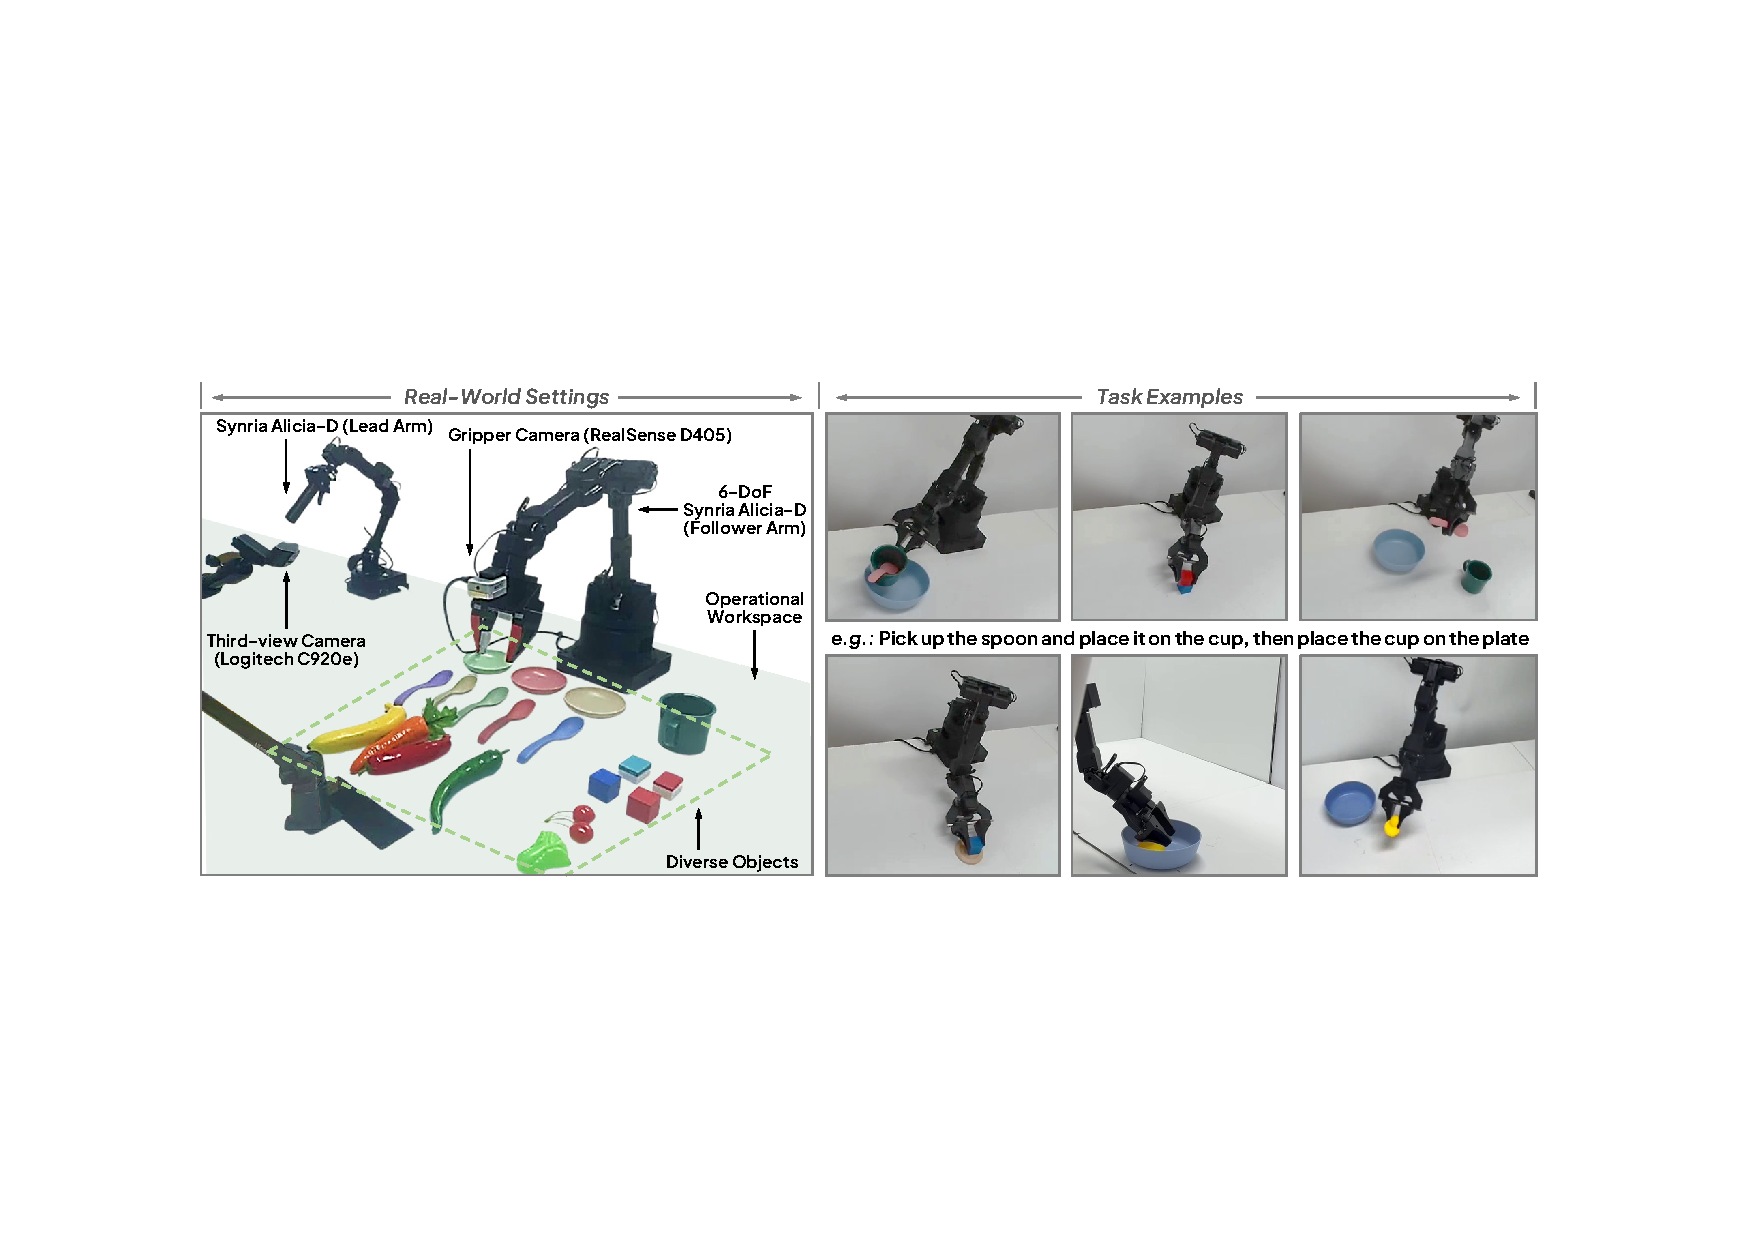
\includegraphics[width=0.95\textwidth]{Figures/real-world1.pdf}	
	\caption{Real-world system Synria Alicia-D and the task examples.}\label{Figure_realworld}
\end{figure} % 





\paragraph{Baselines.}\label{Real-world baselines} 
ACT \citep{ACT-2023} and OFT-style variant \citep{OpenVLA-OFT-2025} are as baselines.

\paragraph{Results.}
The comparison results are shown in Figure \ref{Figure_realworld_results}. Each result is obtained by averaging the results of 10 executions.
Experimental results show that VLA-Adapter has better generalization capabilities in various scenarios. Therefore, VLA-Adapter greatly lowers the barrier to adopting VLA in practical applications. More real-world experiments are detailed in Appendix \ref{AppendixF}.

\begin{figure}[!htbp]
	\centering
	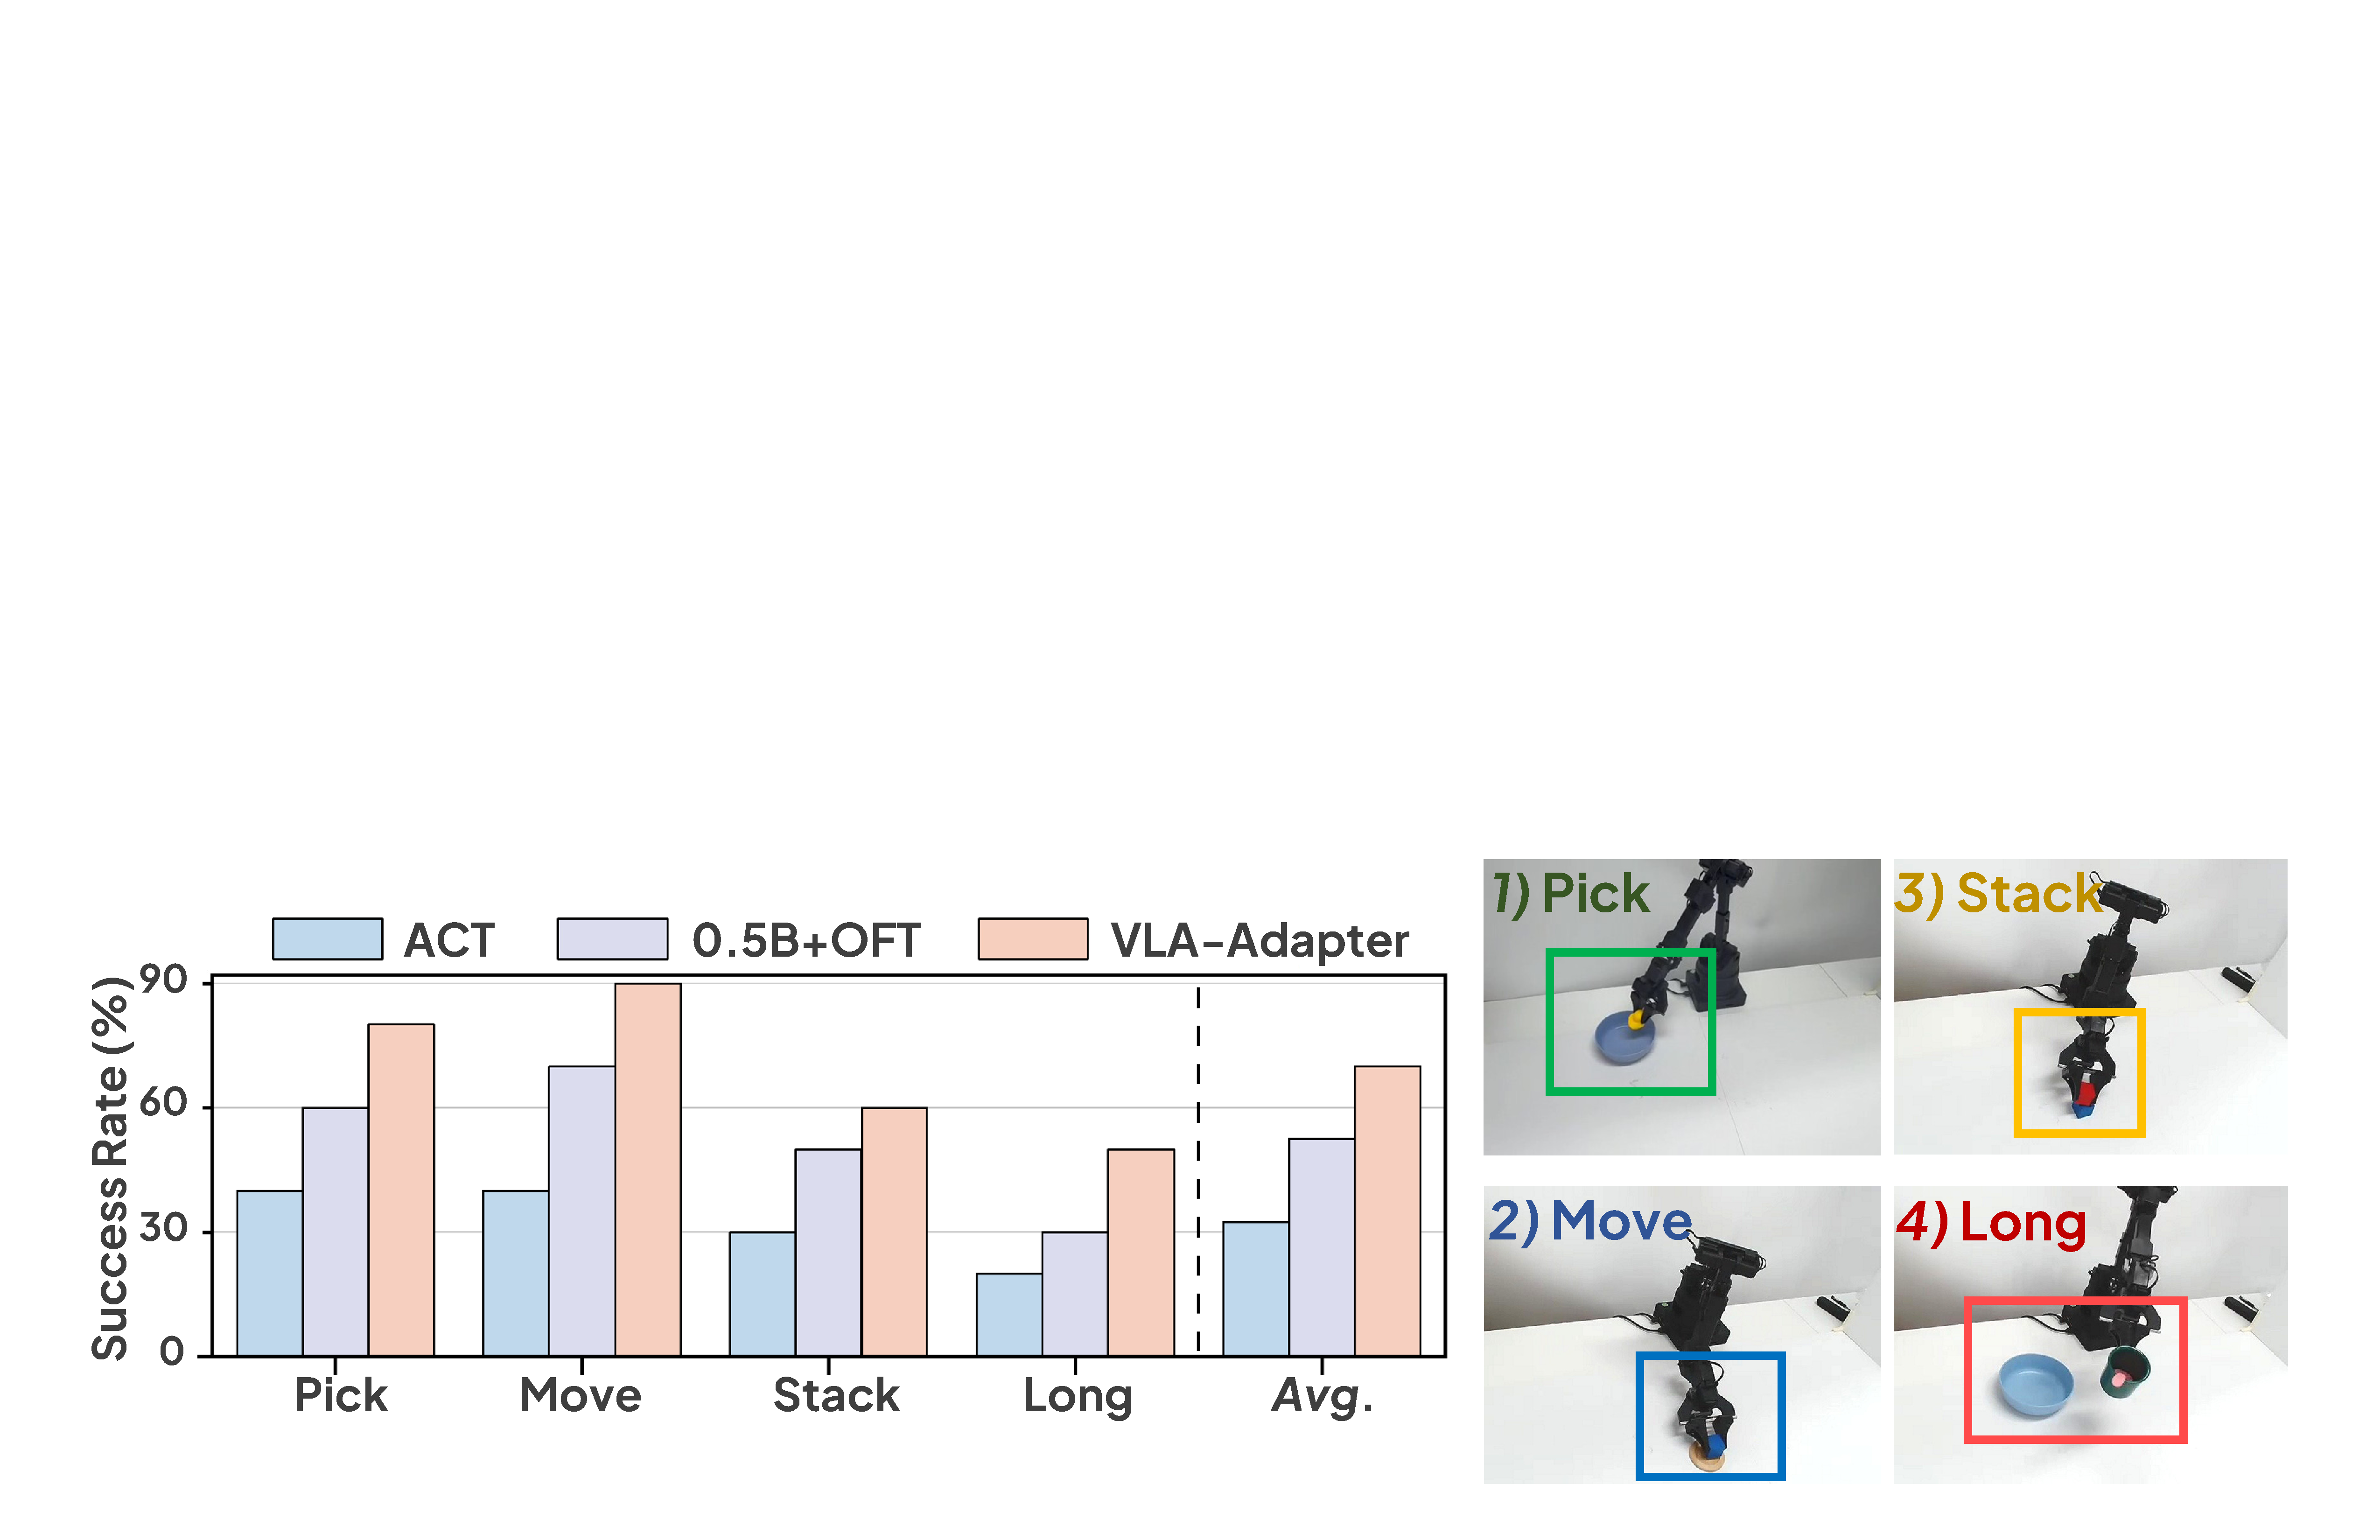
\includegraphics[width=0.87\textwidth]{Figures/realco.pdf}
	\caption{Comparison on real-world tasks.}\label{Figure_realworld_results}
\end{figure}
%

\subsection{Ablation Experiments}\label{sec45}

We explore three key components in the VLA-Adapter: 1. Number of ActionQuery, 2. Condition type, and 3. Injection degree for Policy. The benchmark is LIBERO-Long \citep{LIBERO-2023}.

\paragraph{Number of ActionQuery.}
In our paradigm, the number of ActionQuery is not fixed. To explore the impact of this number on performance, we conducted the following experiments by varying the number of ActionQuery to 1, 4, 8, 16, 64, 128, 256, and 512. The results are shown in Figure \ref{Figure_ActionQuery}. Thus, using too few ActionQuery tokens weakens multimodal aggregation and makes it challenging to condition the Policy. Conversely, employing too many ActionQuery tokens introduces redundancy, interfering with the performance. Therefore, we selected 64 ActionQuery tokens. This number provides the optimal balance between performance and efficiency.

\begin{figure}[!htbp]
	\centering
	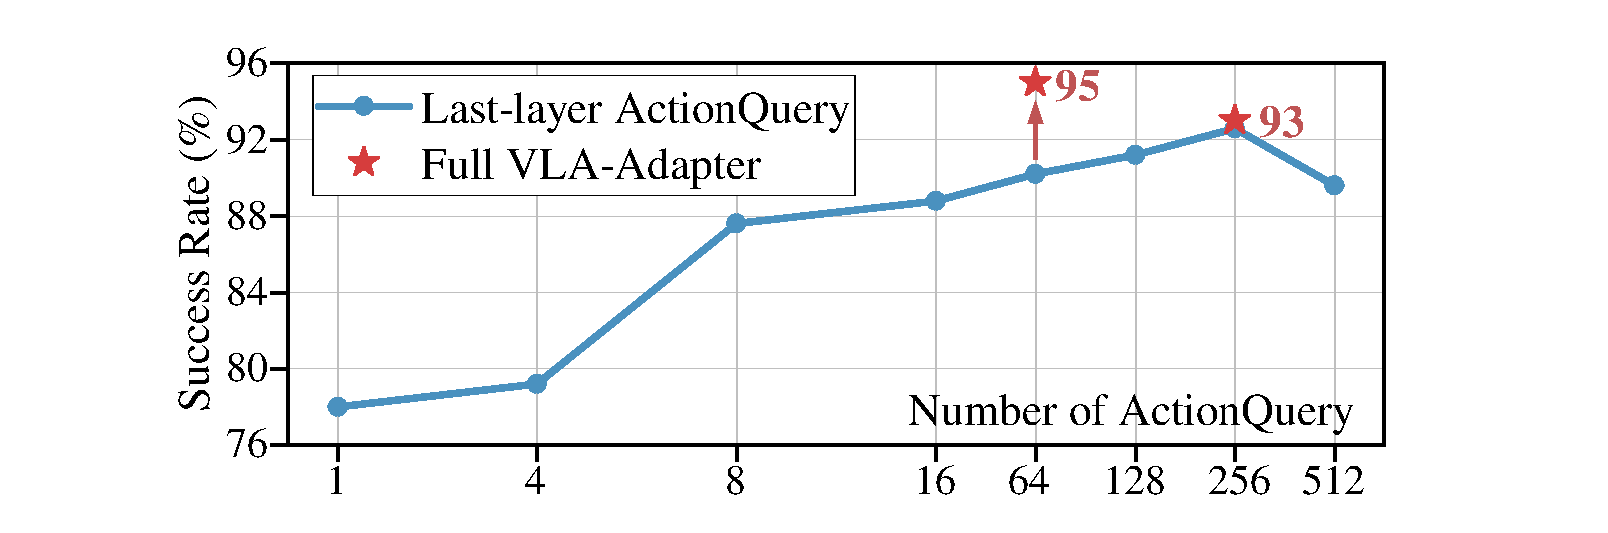
\includegraphics[width=0.63\textwidth]{Figures/ActionQuery.pdf}
	\caption{Comparison of the different numbers of ActionQuery. The blue line shows the result of using only the last-layer ActionQuery. The red star shows the result of the full VLA-Adapter.}\label{Figure_ActionQuery}
\end{figure}


\paragraph{Condition Type.}
In Section \ref{Section_methodology}, we analyzed the overall effects of different conditions on action generation. Here, we present the complete comparison results based on the four classic paradigms in Section \ref{Section_related_work}, as shown in Table \ref{Table_condition_type}. This result demonstrates that using both all-layer Raw and ActionQuery achieves superior performance, indirectly validating the superiority of our bridge paradigm.

\begin{table}[!htbp]
	\centering
	\caption{Comparison with different condition types. The style can be summarized as representative works in Figure \ref{Figure_mapping} of Section \ref{Section_introduction}. ``\textit{N/A}" represents no such method. ``\textbf{Bold}" is the best performance.}\label{Table_condition_type}%
	\begin{tabular}{c|cccc}
		\toprule[1pt]
		Layer  &  Raw   & ActionQuery &Style & \multicolumn{1}{c}{SR $\uparrow$} \\
		\midrule[0.5pt]
		\multicolumn{1}{c|}{\multirow{2}{*}{Last}} & \ding{51}     & \ding{55}      & RoboVLMs \citep{RoboVLMs-2024} & 85.8 \\
		&  \ding{55}     & \ding{51}      & OpenVLA-OFT \citep{OpenVLA-OFT-2025}&90.2 \\
		\midrule[0.5pt] 
		\multicolumn{1}{c|}{\multirow{1}{*}{Intermidiate}} & \ding{51}      & \ding{55}     & GR00T N1 \citep{GR00T-N1-2025} & 88.4 \\
		\midrule[0.5pt] 
		\multicolumn{1}{c|}{\multirow{3}{*}{All}} & \ding{51}      & \ding{55}     &$\pi_0$ \citep{pi0-2025}  &  90.6 \\
		& \ding{55}      & \ding{51}     & \textit{N/A}& 92.6 \\
		\rowcolor[rgb]{ .900,  .900,  .900}& \ding{51}      & \ding{51}     & \textbf{VLA-Adapter (Ours)} & \textbf{95.0} \\
		\bottomrule[1pt]
	\end{tabular}%
\end{table}%

\paragraph{Injection Degree for Policy.}\label{sec453}
In the Bridge Attention, we use learnable parameters to control the injection degree of Raw features $\mathcal{{\cal C}}_t^\mathcal{R}$ and set the injection degree of ActionQuery features $\mathcal{{\cal C}}_t^\mathcal{AQ}$ to 1. Here, we explore other injection degrees, and the comparison results are shown in Table \ref{Table_injection}. Two conclusions can be drawn from the results in Table \ref{Table_injection}:
\textit{From 1) and 2)}, the performance of $\mathcal{{\cal C}}_t^\mathcal{R}$ is inferior to $\mathcal{{\cal C}}_t^\mathcal{AQ}$, so $\mathcal{{\cal C}}_t^\mathcal{R}$ should inject some effective information into Policy through learning.
\textit{From 1) and 4)}, $\mathcal{{\cal C}}_t^\mathcal{AQ}$ aggregates multimodal information, which is beneficial for action generation; it needs to be injected fully into Policy. This result confirms that the Bridge Attention is effective.

\begin{table}[htbp]
	\centering
	\caption{Ablation of other injection degrees.}\label{Table_injection}%
	\begin{tabular}{c|ccc}
		\toprule[1pt]
		&Raw   & ActionQuery    & Success Rate (\%) \\
		\midrule[0.5pt]
		\textit{1)} (\textbf{VLA-Adapter})&$\tanh(g)$  & 1 & \textbf{95.0} \\
		\textit{2)}&1 & 1 & 91.4 \\
		\textit{3)}&1 & $\tanh(g)$  & 91.0 \\
		\textit{4)}&$\tanh(g)$  & $\tanh(g)$  & 92.6 \\
		\bottomrule[1pt]
	\end{tabular}%
\end{table}%